\documentclass{article}
\usepackage[utf8]{inputenc}
\usepackage{indentfirst} 
\setlength{\parindent}{2em}
\usepackage{indentfirst}
\usepackage{graphicx} 
\title{HW4 Scalability: Exchange Matching}
\author{Jichun Shen(js751), Yingzhuo Zhang(yz397)}
\date{March 2018}

\begin{document}

\maketitle              % typeset the title of the contribution

\section{Summary}
%
In this project, we used GO language to program. Considering the exchange matching system need to deal with request concurrently and we want the scalability of our system, GO language supports concurrency at the language level and it has garbage collection. This characteristic makes GO programming language performance very good in this project.
%
We have tables: account table to store account id and the balance for each account; symbol table to store the type of symbols already in our system; acc\_sym table to store the symbol ownership for each account; query table to record each transaction's status; market table to store all currently open transactions for match.
%
\section{Concurrency}
%
The concurrency is implemented by go method which will starts a new goroutine running. We solve the race condition problem by using the build-in lock mechanism in Mysql database. We use 'select ... from ... for update' to lock the tuple we need to do operations on. Preventing other thread to modify this tuple. This tuple will be unlocked when all the operations are finished and commit. In this case, every tuple can only be operated by one thread and tuples which are not involved in this transaction can be accessed and modified by other threads.
%
\section{Scalability Analyze}
%
In this project, the scale of testcase can be show in two dimensions: 
1 size of single xml file;
2 numbers of xml files.
we define a single operation is a operation with one tag such as <account>, <symbol>, <order>, <query>, <cancel>. We have tested time usage for each single operation. The testcases we used are all in testcase0 directory, you can go there for the detail about our measurement of time. The results are presented in Figure 1. The other figure is about dealing with multiple files. We have done test from process 90 files to 140 files and the results are presented in Figure 2, the y-axis is time(s) and x-axis is number of files. The time showed were actually larger than the real processing time because we first used script to generated those files and the generating time were also counted in the result. At very beginning, we just use single thread to deal with it and the result was almost 5 times than what we finally got here. The single thread  result showed in Figure 3\\
%
\begin{figure}[h!]
\centering
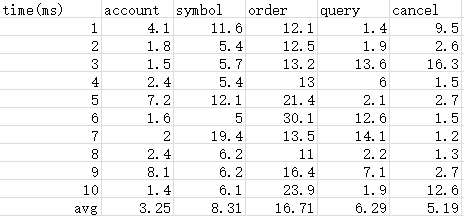
\includegraphics[width=100mm]{spt}
\caption{single operation time usage}
\label{fig:method}
\end{figure}
%

\begin{figure}[h!]
\centering
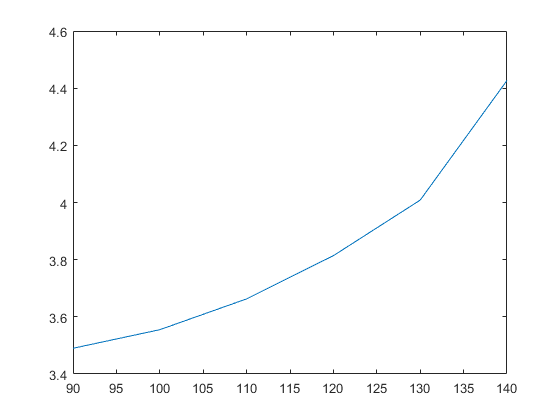
\includegraphics[width=100mm]{mfg}
\caption{multiple files process time usage(multi-threads)}
\label{fig:method}
\end{figure}
\begin{figure}[h!]
\centering
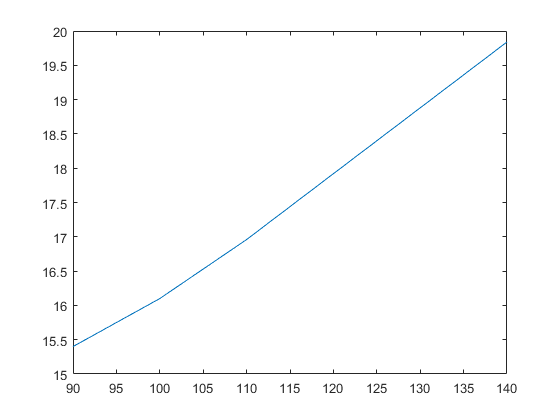
\includegraphics[width=100mm]{sfg}
\caption{multiple files process time usage(single-thread)}
\label{fig:method}
\end{figure}
%
\section{Testcase Instruction}
We offered ten testcases. Each testcase is in a subdirectory and you can run the script to execute it. But there something you should keep in mind when you do the test: 1.read README.txt first 2 restart docker every time you want to run a new testcase offered by us, because the result was designed. For your convenience to quickly know whether the result is right or wrong. We decide to drop table every time you start the program. Therefore, if you don't restart the program, we don't offer right result with several testcase combination. In real life, we don't need to drop all tables when we restart server, but we did here to make testing job easier for you.

%
\end{document}

